\documentclass{article}
\usepackage[portuguese]{babel}
\usepackage[utf8]{inputenc}
\usepackage[margin=1in]{geometry}
\usepackage{graphicx}
\usepackage{biblatex}
\usepackage{csquotes}
\usepackage{float}
\usepackage{titlesec}
\usepackage{array}
\usepackage{tabularx}
\usepackage{hyperref}
\usepackage{fancyhdr}
\usepackage{listings}
\hypersetup{
    colorlinks,
    citecolor=black,
    filecolor=black,
    linkcolor=black,
    urlcolor=black
}
\lstset{
  language=C,                % choose the language of the code
  %numbers=left,                   % where to put the line-numbers
  stepnumber=1,                   % the step between two line-numbers.        
  numbersep=5pt,                  % how far the line-numbers are from the code
  backgroundcolor=\color{white},  % choose the background color. You must add \usepackage{color}
  showspaces=false,               % show spaces adding particular underscores
  showstringspaces=false,         % underline spaces within strings
  showtabs=false,                 % show tabs within strings adding particular underscores
  tabsize=2,                      % sets default tabsize to 2 spaces
  captionpos=b,                   % sets the caption-position to bottom
  breaklines=true,                % sets automatic line breaking
  breakatwhitespace=true,         % sets if automatic breaks should only happen at whitespace
  title=\lstname,                 % show the filename of files included with \lstinputlisting;
}

\setlength{\parindent}{4em}
\setlength{\parskip}{1em}
\renewcommand{\baselinestretch}{1.5}

\pagestyle{fancy}
\fancyfoot{}
\fancyfoot[R]{\thepage}
\addbibresource{references.bib}

\begin{document}

\thispagestyle{empty}

\noindent\begin{minipage}{0.3\textwidth}
    
\includegraphics[scale=0.15]{assets/logo-unicamp.pdf}
\end{minipage}
\hfill
\begin{minipage}{0.6\textwidth}\raggedleft
    UNIVERSIDADE ESTADUAL DE CAMPINAS

    FACULDADE DE TECNOLOGIA DA UNICAMP
    
    SI201 B - Monitoria
    
    Izael Souza
\end{minipage}
\begin{center}
    \hfill%
\end{center}

\begin{center}
    \textbf{\huge Algoritmos de Ordenação}

    \LARGE Implementações em C e explicações dos algoritmos vistos em aula
    
\end{center}

\vspace*{\fill}
\begin{center}
    \textbf{Limeira, SP - Brasil}
    
    \textbf{Novembro 2022}
\end{center}

\thispagestyle{empty}
\renewcommand* \contentsname{Sumário}
\tableofcontents

\section{\textit{Bubble Sort}}

\textit{Bubble Sort} é um dos algoritmos de ordenação mais simples que existe. A ideia dele é iterar sobre uma lista comparando os elementos adjacentes e, caso o primeiro seja maior que segundo, nos fazemos um \textit{swap} (troca), caso queíramos ordenar a lista de forma adjacente.

Apesar de ser o mais simples, não é o mais eficiente. Como estamos comparando elementos adjacentes, nós temos que iterar a lista diversas vezes, comparando os elementos dois-a-dois. Ele é útil em casos onde a lista de elementos não é tão grande.

\subsection{Explicação do Algoritmo}
Nós vamos começar pelo elemento presente no \textit{index} 0 da lista/vetor e vamos comparar com o elemento presente no \textit{index} 1. Caso o primeiro elemento seja maior, nós vamos trocar ele com o segundo elemento. Após isso, nós vamos comparar o elemento do \textit{index} 1 com o elemento no \textit{index} 2. Se for maior, trocamos, caso contrário, apenas seguimos com o algoritmo. Dessa forma, o algoritmo é \textbf{O(n²)}. A imagem abaixo ilustra melhor o funcionamento do algoritmo.
\begin{figure}[H]
    \centering
    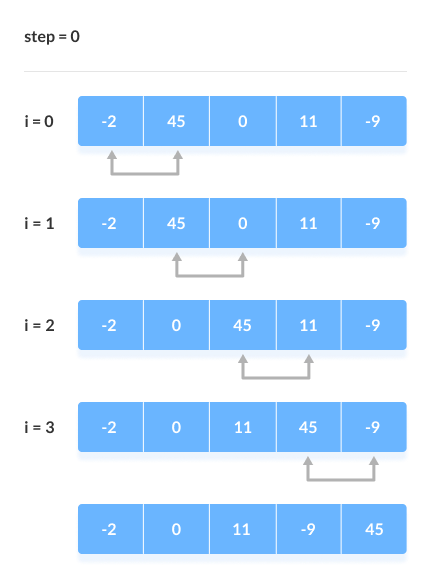
\includegraphics[scale=0.5]{assets/bubble_sort.png}
    \caption{Comparação de elementos adjacentes no \textit{bubble sort}. Fonte: Programiz}
    \label{fig:bubble_sort_0}
\end{figure}

\subsection{Implementação Iterativa}
\begin{lstlisting}[language=C]
void bubbleSort(int* vector, int numberOfElements) {
    while(numberOfElements > 2) {
        for(int i = 0; i < numberOfElements - 1; i++) {
            if(vector[i] > vector[i + 1]) {
                int aux = vector[i];
                vector[i] = vector[i + 1];
                vector[i + 1] = aux
            }
        }
        numberOfElements--;
    }
}
\end{lstlisting}

\subsection{Implementação Recursiva}
\begin{lstlisting}[language=C]
void bubbleSort(int* vector, int numberOfElements) {
    if (numberOfElements < 2)
        return;
    for(int i = 0; i < numberOfElements - 1; i++) {
        if(vector[i] > vector[i + 1]) {
            int aux = vector[i];
            vector[i] = vector[i + 1];
            vector[i + 1] = aux
        }
    }
    bubbleSort(vector, numberOfElements-1);
}
\end{lstlisting}

\subsection{Pontos Importantes}
\begin{itemize}
    \item O \textit{for loop} vai até numberOfElements - 1 pois dentro do \textit{if} fazemos i + 1. Caso o \textit{loop} fosse até numberOfElements, na última posição teríamos um erro pois tentaríamos acessar uma posição que não existe; 
    
    \item Precisamos criar uma variável \textit{aux} para não perdermos o valor de um dos elementos;
\end{itemize}

\section{\textit{Selection Sort}}

\subsection{Explicação do Algoritmo}
\textit{Selection Sort} é um algoritmo de ordenação que roda em tempo O(n²). A ideia por trás dele é \textbf{selecionar} o maior - ou menor, dependendo de como você deseja ordenar - 
valor do conjunto de dados (vetor) e colocá-lo na última posição do vetor. Esse processo se repete com os n - 1 elemetos até os dois últimos.

\subsection{Implementação da Função \textit{max()}}
\begin{lstlisting}[language=C]
int max(int* vector, int size) {
    int max = 0;
    for(int i = 0; i < size; i++) {
        if(vector[i] > max) {
            max = i; // Index of the maximum element
        }
    }
    
    return max;
}
\end{lstlisting}

\subsection{Implementação Iterativa}
\paragraph{Explicação da implementação}
Anteriormente nós definimos a função \textit{max()} para retornarmos o \textbf{índice} do maior elemento. Agora, nós vamos iterar sobre o nosso conjunto de dados (vetor) utilizando
um \textit{while loop}. Dentro do \textit{while}, nós vamos pegar o índice do maior elemento e vamos trocar esse elemento com o que está na última posição. Em seguida, vamos fazer
\textit{numberOfElements - 1}, pois já sabemos que o último elemento é o maior e, portanto, não faz sentido escolhermos um outro \textit{max} e comparar com o último elemento.
\begin{lstlisting}[language=C]
void selecaoIterativo(int* vector, int numberOfElements){
    while(numberOfElements > 1){
        int max = max(vector, numberOfElements);
        // Begin swap
        int aux = vector[max];
        vector[max] = vector[numberOfElements - 1];
        vector[numberOfElements - 1] = aux;
        // End swap
        print(vector, numberOfElements);
        numberOfElements--;
    }
}
\end{lstlisting}

\subsection{Implementação Recursiva}
\begin{lstlisting}[language=C]
void selecaoRecursivo(int* vector, int numberOfElements){
    if(numberOfElements < 2){
        return;
    }
    int max = max(vector, numberOfElements);
    int aux = vector[max];
    vector[max] = vector[numberOfElements - 1];
    vector[numberOfElement - 1] = aux;
    print(vector, numberOfElements);
    selecaoRecursivo(vector, numberOfElements - 1);
}
\end{lstlisting}

\section{\textit{Insertion Sort}}

\subsection{Explicação do Algoritmo}
A melhor analogia a ser fazer quando falamos de \textit{Insertion Sort} é um jogo de cartas. Você começa com a mão vazia e, conforme for recebendo as cartas, você as adiciona
\textbf{em ordem} na sua mão, comparando essa nova carta com as que já estão na sua mão. Nós vamos iterar o conjunto de dados (vetor) e vamos comparar com os elementos anteriores.
Se ele for menor, nós vamos dar um \textit{shift} em todos os elementos a partir da posição onde queremos colocar esse elemento. Esse processo vai ser repetido até o vetor estar
totalmente ordenado.

\subsection{Implementação Iterativa}
\paragraph{Explicação}
Nós começamos definindo uma variável \textit{lixo} e uma variável \textit{n}. A primeira será usada para sabermos onde vamos \textbf{inserir} o novo elemento. A segunda
variável define o tamanho do \textit{subarray} com o qual vamos trabalhar (inicialmente 2). Enquanto o tamanho do \textit{subarray} for menor ou igual ao tamanho do \textit{array} original, nós vamos:
\begin{itemize}
  \item Definir uma variável \textit{aux} com o valor do último elemento do \textit{subarray};
  \item Colocar o valor \textit{lixo} (-1) na última posição do \textit{subarray};
  \item Definir uma variável \textit{i}, que representa onde vamos começar nossa ordenação. Primeiramente vamos começar ordenando da posição 0 e depois da posição 1, e assim por diante.
    Podemos fazer isso pois já sabemos que os elementos anteriores estão ordenados;
  \item Criar um \textit{while loop} que vai rodar enquanto o valor de \textit{i} for maior ou igual a zero e o elemento na posição \textit{i} for maior que \textit{aux}. Dentro desse \textit{loop}
    vamos movendo o valor -1 para a esquerda. A partir do momento que descobrirmos que \textit{aux} é menor que o elemento que estamos, vamos colocá-lo naquela posição.
\end{itemize}

\begin{lstlisting}[language=C]
void insercaoIterativo(int* vector, int numberOfElements){
    int lixo = -1;
    int n = 2;
    while(n <= numberOfElements){
        int aux = vector[n - 1];
        vector[n - 1] = lixo;
        int i = n - 2;
        print(vector, n);
        while(i >= 0 && vector[i] > aux) {
            vector[i + 1] = vector[i];
            vector[i] = lixo;
            i--;
            print(vector, n);
        }
        vector[i + 1] = aux;
        print(vector, n);
        n++;
    }
}

\end{lstlisting}

\paragraph{Exemplo}
Com o objetivo de facilitar a visualização, vamos aplicar esse algoritmo a um vetor. No caso, o vetor em questão será de tamanho 6 e composto pelos seguintes elementos na seguinte ordem:
\{9, 8, 2, 3, 5, 6\}. Chamando esta função (\textit{insercaoIterativo(vetor, 6)}), nós temos o \textit{output}:

[9,-1](2)

[-1,9](2)

[8,9](2)

[8,9,-1](3)

[8,-1,9](3)

[-1,8,9](3)

[2,8,9](3)

[2,8,9,-1](4)

[2,8,-1,9](4)

[2,-1,8,9](4)

[2,3,8,9](4)

[2,3,8,9,-1](5)

[2,3,8,-1,9](5)

[2,3,-1,8,9](5)

[2,3,5,8,9](5)

[2,3,5,8,9,-1](6)

[2,3,5,8,-1,9](6)

[2,3,5,-1,8,9](6)

[2,3,5,6,8,9](6)

\subsection{Implementação Recursiva}
\paragraph{Explicação}
A ideia por trás do algoritmo recursivo é a mesma do iterativo. A única diferença é que ao invés de usarmos dois \textit{while loops}, usamos apenas um. Aqui, nós vamos chamar a função
dentro dela mesma mudando apenas o parâmetro \textit{numberOfElements}, pois queremos dividir o nosso \textit{array} original em vários \textit{subarrays} e ordenar eles. O nosso caso
base, ou seja, o nosso caso de parada, é quando o \textit{numberOfElements} for menor que 2.

\begin{lstlisting}[language=C]
void insercaoRecursivo(int* vector, int numberOfElements){
    int lixo = -1;
    if(numberOfElements < 2)
        return;

    insercaoRecursivo(vector, numberOfElements - 1)
    int aux = vector[n - 1];
    int n = 2;
    int i = n - 2;
    print(vector, n);
    
    while(i >= 0 && vector[i] > aux) {
        vector[i + 1] = vector[i];
        vector[i] = lixo;
        i--;
        print(vector, n);
    }
    vector[i + 1] = aux;
    print(vector, n);
}
\end{lstlisting}

\section{\textit{Merge Sort}}

\subsection{Explicação do Algoritmo}
O algoritmo \textit{Merge Sort} é um algoritmo do tipo \textit{Divide and Conquer}, ou seja, dividir e conquistar. Nós vamos dividir nosso problema
em problemas menores e resolver esses problemas menores primeiro. Dado um \textit{array}, nós vamos dividir ele em duas metades até chegarmos em um ponto
no qual não será mais possível dividí-lo (vazio ou com um elemento). Em cada \textit{subarray}, nós vamos chamar o \textit{mergesort} para ordená-los.
Depois que as metades forem ordenadas, nós vamos juntar elas (\textit{merge}), reconstruindo nosso \textit{array} original. O funcionamento do algoritmo está representado de forma visual
no diagrama abaixo.

\begin{figure}[H]
    \centering
    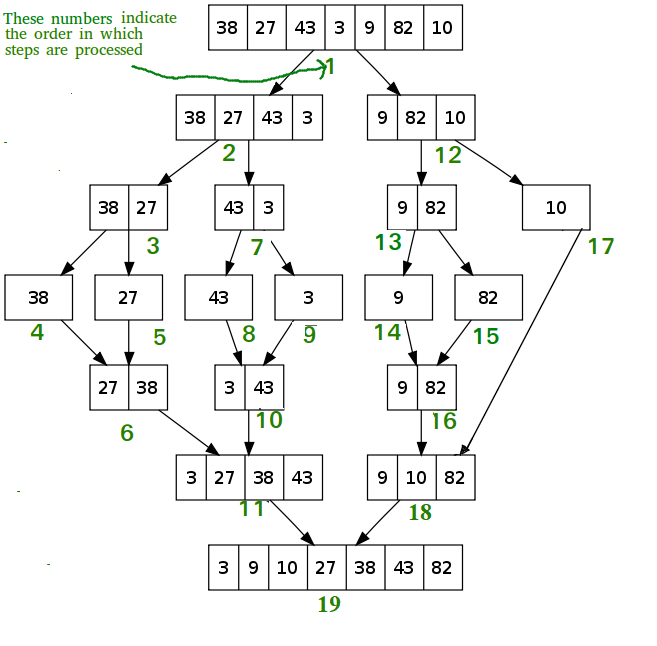
\includegraphics[scale=0.6]{assets/mergesort_diagram.png}
    \caption{Diagrama do funcionamento do \textit{merge sort}. Fonte: GeeksforGeeks}
    \label{fig:merge_sort_0}
\end{figure}

\subsection{Função \textit{merge()}}
\paragraph{Explicação}
Essa função é reponsável por juntar os \textit{subarrays} ordenados. Nós temos 5 parâmetros: um vetor que corresponde a uma das metades de um vetor maior, o tamanho desse vetor,
um vetor que corresponde a outra metade do vetor maior, o tamanho desse vetor, e o vetor original. Nós definimos três variáveis \textit{top}, cada uma referente a um vetor dos três
mencionados anteriormente, e inicializamos elas para 0.

Em seguida, nós vamos fazer um \textit{while loop} enquanto o \textit{top1} for menor que \textit{n1} e \textit{top2} for menor que \textit{n2}. Dentro desse \textit{loop}, nós
vamos comparar os elementos de ambas as metades e colocar as mesmas em ordem no vetor original \footnote{Note que estamos usando \textit{top++}. Primeiro eu acesso o valor do
\textit{top} naquele momento - por exemplo 3 -  e depois eu incremento - nesse caso para 4.}. Os dois últimos \textit{while} servem para copiar elementos restantes caso haja algum.

\begin{lstlisting}[language=C]
void merge(int *v1,int n1,int *v2,int n2,int *v){
    int top1=0,top2=0,top=0;
    while(top1<n1&&top2<n2){
        if(v1[top1]<v2[top2]){
            v[top++]=v1[top1++];
        }else{
            v[top++]=v2[top2++];
        }
    }
    while(top1<n1){
        v[top++]=v1[top1++];
    }
    while(top2<n2){
        v[top++]=v2[top2++];
    }
}

\end{lstlisting}

\subsection{Função \textit{mergesort()}}
\paragraph{Explicação}
Dado um vetor de tamanho \textit{n}, nós vamos dividí-lo em dois até não ser mais possível, ou seja, até que o seu tamanho seja 0 ou 1. Definimos duas variáveis \textit{n1} e \textit{n2}
que armazenam o tamanho da primeira metade do \textit{array} e o tamanho da segunda metade do \textit{array}. Depois disso, vamos chamar a função \textit{merge()} para juntar os arrays
na ordem certa.

\begin{lstlisting}[language=C]
void mergeSort(int v[],int n){
    if(n>1){
        int n1,n2;
        n1 = n/2;
        n2 = n-n1;
        int *v1,*v2;
        v1 = (int *)malloc(sizeof(int)*n1);
        v2 = (int *)malloc(sizeof(int)*n2);

        for(int i=0;i<n1;i++){
            v1[i]=v[i];
        }
        for(int i=0;i<n2;i++){
            v2[i]=v[n1+i];
        }

        mergeSort(v1,n1);
        mergeSort(v2,n2);
        merge(v1,n1,v2,n2,v);
        free(v1);
        free(v2);
    }
}
\end{lstlisting}



\addtocontents{toc}{\protect\thispagestyle{empty}}
\pagenumbering{gobble}
\fancyhead{}
\printbibliography[heading=bibintoc, title={Referências}]


\end{document}

